\documentclass{beamer}

\usepackage{polski}
\usepackage[utf8]{inputenc}
\usepackage{graphics}
\usetheme{Warsaw}

\title{Drag Reduction System}
\subtitle{DRS}
\author{Mateusz Iwańczak}
\date{\today}

\begin{document}
\begin{frame}
\titlepage
\end{frame}

\begin{frame}{Wstęp}
\centering
\begin{itemize}
\item Pasjonaci królowej sportów motorowych, którymi określa się Formułę 1, śledzą wydarzenia wokół niej na bieżąco.
\item Są tacy, którzy oglądają jedynie wyścig na ekranie telewizora lub monitora.
\item Znajdą się też ci, którzy interesują się nowinkami technologicznymi.
\item Na osiągi bolidu wpływają nie tylko umiejętności kierowcy i jednostki napędowe.
\item Wpływają na nie również cechy konstrukcyjne.
\item System DRS jest jedną ze składowych konstrukcyjnych.
\item Jest jedną z nowinek technicznych, która wpłynęła na historię tej dyscypliny.
\end{itemize}
\end{frame}

\begin{frame}{DRS - definicja}
\centering
\begin{itemize}
\item Na początek warto sformułować definicje tegoż systemu, bo istotnie nim jest.
\end{itemize}
\begin{block}{DRS}
System został rozpowszechniony w 2011 roku. Ułatwiał zadanie wyprzedzenia rywala, lecz tylko w wyznaczonej do tego strefie na torze.
\end{block}
\end{frame}

\begin{frame}{Postać DRS}
\begin{figure}[h]
\centering
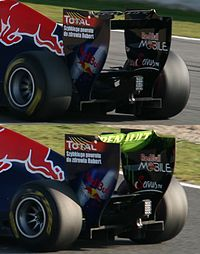
\includegraphics[width=5cm]{./images/DRS3}
\caption[1]{Zastosowanie DRS w bolidzie Red Bull RB7}
\end{figure}
\end{frame}

\begin{frame}{Zastosowanie systemu}
\centering
\begin{block}{Dla pasjonatów}
Zawsze ważne jest zastosowanie każdej nowinki w praktyce
\end{block}
\begin{alertblock}{UWAGA 1}
DRS jest możliwy do użycia dopiero po trzech okrążeniach!
\end{alertblock}
\begin{alertblock}{UWAGA 2}
DRS zawsze jest wyłączony, gdy samochód bezpieczeństwa (Safety Car) jest obecny na torze!
\end{alertblock}
\end{frame}

\begin{frame}{Zastosowanie systemu c.d.}
\centering
\begin{alertblock}{UWAGA 3}
Drag Reduction System ma status włączonego trzy okrążenia po zjeździe Safety Car'u, gdy warunki pogodowe są ocenione jako dobre.
\end{alertblock}
\begin{exampleblock}{Opcja}
Kierowca ma możność skorzystania z niego, gdy znajduje się w dystansie nie większym niż jedna sekunda do rywala.
\end{exampleblock}
\begin{block}{Info}
Są wyznaczone strefy dla tego rozwiązania. Są to zazwyczaj długie proste.
\end{block}
\end{frame}

\begin{frame}{Manewr wyprzedzania z DRS}
\begin{figure}[h]
\centering
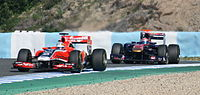
\includegraphics[width=10cm]{./images/DRS2}
\caption[2]{Virgin MVR-02 i Toro Rosso STR6 z aktywowanym systemem DRS}
\end{figure}
\end{frame}

\begin{frame}{Zastosowanie systemu c.d.}
\centering
\begin{block}{Warto zapamiętać}
Kierowca, stosując go, ma korzyść w postaci mniejszego oporu powietrza. To z kolei oznacza potencjalnie większą prędkość, co w konsekwencji prowadzi do łatwiejszego manewru wyprzedzania.
\end{block}
\begin{exampleblock}{Info}
Dezaktywacja patentu następuje w momencie hamowania bolidu, czyli naciśnięcia pedału hamowania.
\end{exampleblock}
\begin{alertblock}{Uwaga 4}
Złe warunki pogodowe wykluczają używanie DRS.
\end{alertblock}
\end{frame}

\begin{frame}{Bibliografia}
\centering
\begin{enumerate}
\item https://pl.wikipedia.org/wiki/Drag\_Reduction\_System
\item https://upload.wikimedia.org/wikipedia/commons/thumb/9/ \\ 9b/RB7\_adjustable\_rear\_wing.jpg/200px-RB7\_adjustable \\ \_rear\_wing.jpg
\item https://upload.wikimedia.org/wikipedia/commons/thumb/9/ \\ 9e/F1\_2011\_Jerez\_day\_3-16.jpg/200px-F1\_2011\_Jerez\_day\_3- \\ 16.jpg
\end{enumerate}
\end{frame}
\end{document}